% Provenance (never printed): see sources/outline_sources.md (Year 2: interstellar
% medium, molecular clouds, gravitational collapse and the Jeans criterion, protostars
% and protostellar discs). Curves from figdata/bachelor-2/jeans.py; exercise and problem
% values in the Book 4 scratch calculator calc/ch01.py.
\chapter{Medium Antarbintang dan Pembentukan Bintang}\label{ch:b2:ism-star-formation}

Di rasi Taurus, sekitar \qty{140}{\parsec} dari Matahari, sebuah bercak gelap
menutupi bintang-bintang di belakangnya. Jika diamati dengan teleskop radio yang
disetel pada garis-garis karbon monoksida, bercak itu ternyata awan gas dingin
yang massanya sekitar dua puluh ribu kali massa Matahari, penuh dengan filamen;
di dalam simpul-simpulnya yang paling padat, bintang-bintang muda sedang lahir,
dan di sekitar salah satunya, HL Tauri, sebuah cakram debu memperlihatkan pola
cincin terang dan gelap tempat planet-planet mungkin sudah mulai terbentuk.
Matahari, Bumi, dan setiap atom dalam batuan buku ini dahulu berada di dalam awan
semacam itu. Bab ini mengikuti materi sebuah sistem planet dari gas tipis di
antara bintang-bintang hingga cakram di sekitar bintang yang baru lahir: dari apa
\omterm{def:b2:ism-star-formation:ism}{medium antarbintang} tersusun, mengapa awan yang ditopang oleh panasnya sendiri
akhirnya runtuh, berapa lama keruntuhan itu berlangsung, bagaimana sebuah bintang
menghimpun massanya, dan mengapa materi yang gagal jatuh ke dalamnya berakhir
sebagai cakram.

\begin{recall}
Bintang di deret utama bersinar dengan memfusikan hidrogen menjadi helium di
intinya dan menopang dirinya dengan tekanannya melawan beratnya sendiri;
kedudukannya pada diagram Hertzsprung--Russell ditentukan oleh massanya (fisika,
Sarjana Tahun ke-3). Benda pada orbit tertutup di sekitar massa $M$ mematuhi hukum
ketiga Kepler, $T^2 = 4\pi^2 a^3/(GM)$ (fisika, Sarjana Tahun ke-1). Benda hitam
bersuhu $T$ memancarkan $\sigma T^4$ per satuan luas (fisika, Sarjana
Tahun ke-2). Dalam gas ideal yang terdiri atas $N$ partikel, energi kinetik
translasi rata-ratanya adalah $\tfrac32 N k_{\mathrm B} T$. Parsek,
\qty{3.086e16}{m}, adalah satuan jarak volume Tahun 1.
\end{recall}

\section{Materi di antara bintang-bintang}

Ruang di antara bintang-bintang tidaklah kosong. Di dekat Matahari, ruang itu
rata-rata berisi sekitar satu atom hidrogen per sentimeter kubik, yaitu massa jenis
\qty{2.7e-24}{g.cm^{-3}}; udara yang kita hirup berisi sekitar $10^{19}$ kali lebih
banyak molekul dalam volume yang sama (\cref{exo:b2:ism-star-formation:1}). Tersebar di seluruh Galaksi, materi tipis
ini tetap mencapai \qtyrange{10}{15}{\percent} massa
cakram Galaksi.
% ledger: ferriere:mean-density, ferriere:disc-fraction

\begin{definition}[Medium antarbintang, debu antarbintang]
\label{def:b2:ism-star-formation:ism}
Yang disebut \emph{medium antarbintang}\index{medium antarbintang} adalah gas dan debu
yang mengisi ruang di antara bintang-bintang sebuah galaksi. Yang disebut \emph{debu
antarbintang}\index{debu antarbintang} adalah bagiannya yang berupa butiran padat,
berukuran dari beberapa nanometer hingga sekitar satu mikrometer, yang tersusun atas
silikat, senyawa karbon, dan, di daerah yang dingin, es.
\end{definition}

Komposisinya sama dengan yang diukur pada Matahari dan pada meteorit: menurut massa,
\qty{70.4}{\percent} hidrogen, \qty{28.1}{\percent} helium, dan
\qty{1.5}{\percent} unsur yang lebih berat. Hanya \qtyrange{0.5}{1}{\percent}
massanya berupa debu, tetapi debu itu menyimpan sebagian besar beberapa unsur: gasnya
lebih miskin magnesium, silikon, dan besi daripada Matahari dengan faktor 10 hingga 100,
karena atom-atom itu terkunci di dalam butiran, sedangkan karbon, nitrogen, dan oksigen
hanya berkurang dengan faktor 1.2 hingga 3. Butiran-butiran itu adalah zat padat pertama
sebuah sistem planet yang kelak terbentuk; \cref{ch:b2:planet-formation-meteorites}
mengikuti perjalanannya.
% ledger: ferriere:composition, ferriere:dust-fraction, ferriere:refractory-depletion

\subsection{Lima fase}

Gas itu jauh dari seragam. Ia hadir dalam beberapa keadaan yang berbeda, atau fase,
masing-masing dengan rentang suhu dan kerapatannya sendiri (tabel di bawah). Sekitar
separuh massanya berada di awan-awan yang hanya mengisi \qtyrange{1}{2}{\percent} volume;
sisanya, yang hangat atau panas, mengisi ruang di antara awan-awan itu.
% ledger: ferriere:disc-fraction

\begin{table}[htbp]
\centering
\small
\begin{tabular}{lll}
\hline
fase & suhu (K) & kerapatan $n$ (\unit{cm^{-3}}) \\
\hline
molekul & 10--20 & $10^2$--$10^6$ \\
atom dingin & 50--100 & 20--50 \\
atom hangat & 6000--10\,000 & 0.2--0.5 \\
terionisasi hangat & sekitar 8000 & 0.2--0.5 \\
terionisasi panas & sekitar $10^6$ & sekitar 0.0065 \\
\hline
\end{tabular}
\caption{Fase-fase gas antarbintang di dekat Matahari; $n$ adalah kerapatan jumlah
inti hidrogen.}
\label{tab:b2:ism-star-formation:phases}
% ledger: ferriere:molecular, ferriere:cold-atomic, ferriere:warm-atomic, ferriere:warm-ionized, ferriere:hot-ionized
\end{table}

Tabel itu menyembunyikan suatu keteraturan. Tekanan gas ideal adalah
$P = n k_{\mathrm B} T$, sehingga hasil kali $nT$ mengukurnya. Untuk gas atom dingin,
$nT$ sekitar $30\times75 \approx 2000$ (dalam \unit{K.cm^{-3}}), untuk gas atom
hangat sekitar $0.3\times8000 \approx 2400$, untuk gas panas sekitar
$0.0065\times10^6 = 6500$: dalam batas faktor beberapa kali, ketiga fase yang
berbagi ruang di antara awan-awan itu bertekanan sama (gambar di bawah).
Di tempat gas panas dan gas dingin bersentuhan pada tekanan yang sama, tidak ada yang
mendorong yang lain menjauh; gas yang mendingin pada tekanan tetap menjadi lebih rapat
sebanding dengan pendinginannya dan turun dari fase hangat ke fase dingin. \omterm{def:b2:ism-star-formation:molecular-cloud}{Awan molekul} mencapai tekanan yang jauh lebih tinggi, hingga ribuan kali lipat di bagian-bagiannya yang padat: awan itu disatukan oleh gravitasinya sendiri, bukan oleh
tekanan lingkungannya.

\begin{omfigure}
\begin{tikzpicture}
\begin{axis}[omrecord, width=0.86\linewidth, height=6.4cm, xmode=log, ymode=log,
  xmin=1e-3, xmax=1e7, ymin=3, ymax=3e6,
  xlabel={kerapatan inti hidrogen $n$ (\unit{cm^{-3}})}, ylabel={suhu $T$ (K)},
  tick label style={font=\scriptsize}, label style={font=\small}, clip=false,
  legend pos=north east, legend style={font=\scriptsize, draw=black!30}]
\addplot[black!45, densely dashed, domain=1e-3:1e3, samples=2] {3000/x};
\addlegendentry{$nT = \num{3000}$}
\addplot[black!60, densely dotted, thick, domain=0.1:1e5, samples=2] {3e5/x};
\addlegendentry{$nT = 3\times10^5$}
\fill[blue!45, opacity=0.6] (axis cs:1e2,10) rectangle (axis cs:1e6,20);
\fill[teal!50, opacity=0.6] (axis cs:20,50) rectangle (axis cs:50,100);
\fill[orange!55, opacity=0.6] (axis cs:0.2,6000) rectangle (axis cs:0.5,10000);
\fill[red!45, opacity=0.6] (axis cs:0.2,5714) rectangle (axis cs:0.5,11200);
\fill[violet!50, opacity=0.6] (axis cs:0.00464,7.14e5) rectangle (axis cs:0.0091,1.4e6);
\node[font=\scriptsize, anchor=south east] at (axis cs:1e6,20) {awan molekul};
\node[font=\scriptsize, anchor=south west] at (axis cs:50,100) {atom dingin};
\node[font=\scriptsize, anchor=east, align=right] at (axis cs:0.17,8000) {atom hangat\\dan terionisasi hangat};
\node[font=\scriptsize, anchor=west] at (axis cs:0.011,1e6) {terionisasi panas};
\end{axis}
\end{tikzpicture}

\par\smallskip{\small Fase-fase gas antarbintang di dekat Matahari (rentang-rentang pada tabel
di atas; fase terionisasi hangat dan fase panas, yang diberikan sebagai nilai tunggal, digambar
sebagai kotak selebar faktor 1.4). Di sepanjang setiap garis kelabu, tekanan $nk_{\mathrm B}T$
tetap: fase dingin, hangat, dan panas terletak dekat pada tekanan yang sama, dalam batas faktor
beberapa kali, sedangkan \omterm{def:b2:ism-star-formation:molecular-cloud}{awan molekul}, yang terikat oleh gravitasinya sendiri, mencapai tekanan hingga ribuan kali lebih tinggi.
Data: Ferrière (2001).}
\end{omfigure}

Debu menampakkan dirinya dengan tiga cara. Debu meredupkan cahaya bintang di
belakangnya, dan meredupkan cahaya biru lebih kuat daripada cahaya merah, sehingga
bintang yang terlihat melaluinya tampak lebih merah daripada sebenarnya. Debu bersinar
dalam inframerah jauh dan pada panjang gelombang milimeter, pada suhu beberapa puluh
kelvin yang dicapainya karena dihangatkan cahaya bintang. Dan debu menyembunyikan apa pun
yang ada di dalam awan padat dari teleskop optik; itulah sebabnya pembentukan bintang
diamati pada panjang gelombang radio dan inframerah. Gas dilacak melalui garis-garisnya:
hidrogen atom melalui garis radionya pada \qty{21}{cm}, hidrogen molekul, yang hampir
tidak memancar ketika dingin, melalui garis-garis molekul yang menyertainya, terutama karbon monoksida.

\section{Awan molekul}

Fase yang paling dingin dan paling padat adalah tempat bintang terbentuk.

\begin{definition}[Awan molekul, inti padat]
\label{def:b2:ism-star-formation:molecular-cloud}
Yang disebut \emph{awan molekul}\index{awan molekul} adalah daerah \omterm{def:b2:ism-star-formation:ism}{medium
antarbintang} yang cukup padat dan buram sehingga hidrogennya sebagian besar berupa
molekul, \ce{H2}, yang terlindung oleh debu dari cahaya ultraungu bintang-bintang
yang akan memecahnya; suhunya sekitar \qty{10}{K} hingga \qty{20}{K}. Yang disebut
\emph{inti padat}\index{inti padat} adalah kondensasi yang kompak di dalam awan
molekul, berdiameter beberapa persepuluh parsek atau kurang, dengan kerapatan
$10^4$ hingga $10^5$ partikel per sentimeter kubik, yang darinya terbentuk satu bintang
atau sekelompok kecil bintang.
\end{definition}

Awan-awan tersusun dalam suatu hierarki (tabel di bawah). Awan gelap seperti Taurus
berisi gumpalan, dan gumpalan berisi inti, setiap tingkat lebih padat, lebih kecil, dan
lebih tenang daripada tingkat di atasnya: di dalam inti, gas bergerak paling cepat beberapa
persepuluh kilometer per sekon, yaitu laju bunyi dalam gas bersuhu \qty{10}{K}. Daerah
Taurus yang dipetakan dalam karbon monoksida berisi gas sekitar \num{2.4e4} massa
Matahari; hanya \qtyrange{0.3}{1.2}{\percent} darinya yang telah menjadi bintang-bintang
muda yang terlihat di sana, dengan laju sekitar delapan bintang setiap seratus ribu
tahun selama tiga juta tahun terakhir. Pembentukan bintang berlangsung lambat dan boros.
% ledger: bt07:clouds, bt07:clumps, bt07:cores, goldsmith:taurus-mass, goldsmith:taurus-sfe, goldsmith:taurus-distance

\begin{table}[htbp]
\centering
\small
\begin{tabular}{lccc}
\hline
 & awan gelap & gumpalan & \omterm{def:b2:ism-star-formation:molecular-cloud}{inti padat} \\
\hline
massa (massa Matahari) & $10^3$--$10^4$ & 50--500 & 0.5--5 \\
ukuran (pc) & 2--15 & 0.3--3 & 0.03--0.2 \\
kerapatan rata-rata (\unit{cm^{-3}}) & 50--500 & $10^3$--$10^4$ & $10^4$--$10^5$ \\
suhu gas (K) & sekitar 10 & 10--20 & 8--12 \\
contoh & Taurus, Musca & --- & L1544, B68 \\
\hline
\end{tabular}
\caption{Hierarki sebuah \omterm{def:b2:ism-star-formation:molecular-cloud}{awan molekul} gelap. Kerapatan menghitung semua
partikel. Data: Bergin dan Tafalla (2007).}
\label{tab:b2:ism-star-formation:hierarchy}
% ledger: bt07:clouds, bt07:clumps, bt07:cores
\end{table}

Mengapa awan-awan itu begitu dingin? Gas kehilangan energi dengan memancarkan foton yang
lolos, dan molekul adalah pemancar yang efisien: sebuah tumbukan menaikkan molekul karbon
monoksida ke tingkat rotasi yang lebih tinggi, molekul itu kembali turun dengan
memancarkan foton pada panjang gelombang milimeter, dan foton itu meninggalkan awan,
membawa serta energi tumbukan tersebut. Debu, yang dihangatkan oleh cahaya bintang redup
yang masuk, memancar dalam inframerah jauh. Pemanasannya, oleh sinar kosmik dan oleh
cahaya bintang yang tersaring debu, lemah; keseimbangannya tercapai di dekat
\qty{10}{K}. Dalam gas semacam itu tekanan termalnya kecil, dan gravitasi dapat
menang.

\begin{omfigure}
\begin{minipage}[c]{0.44\linewidth}
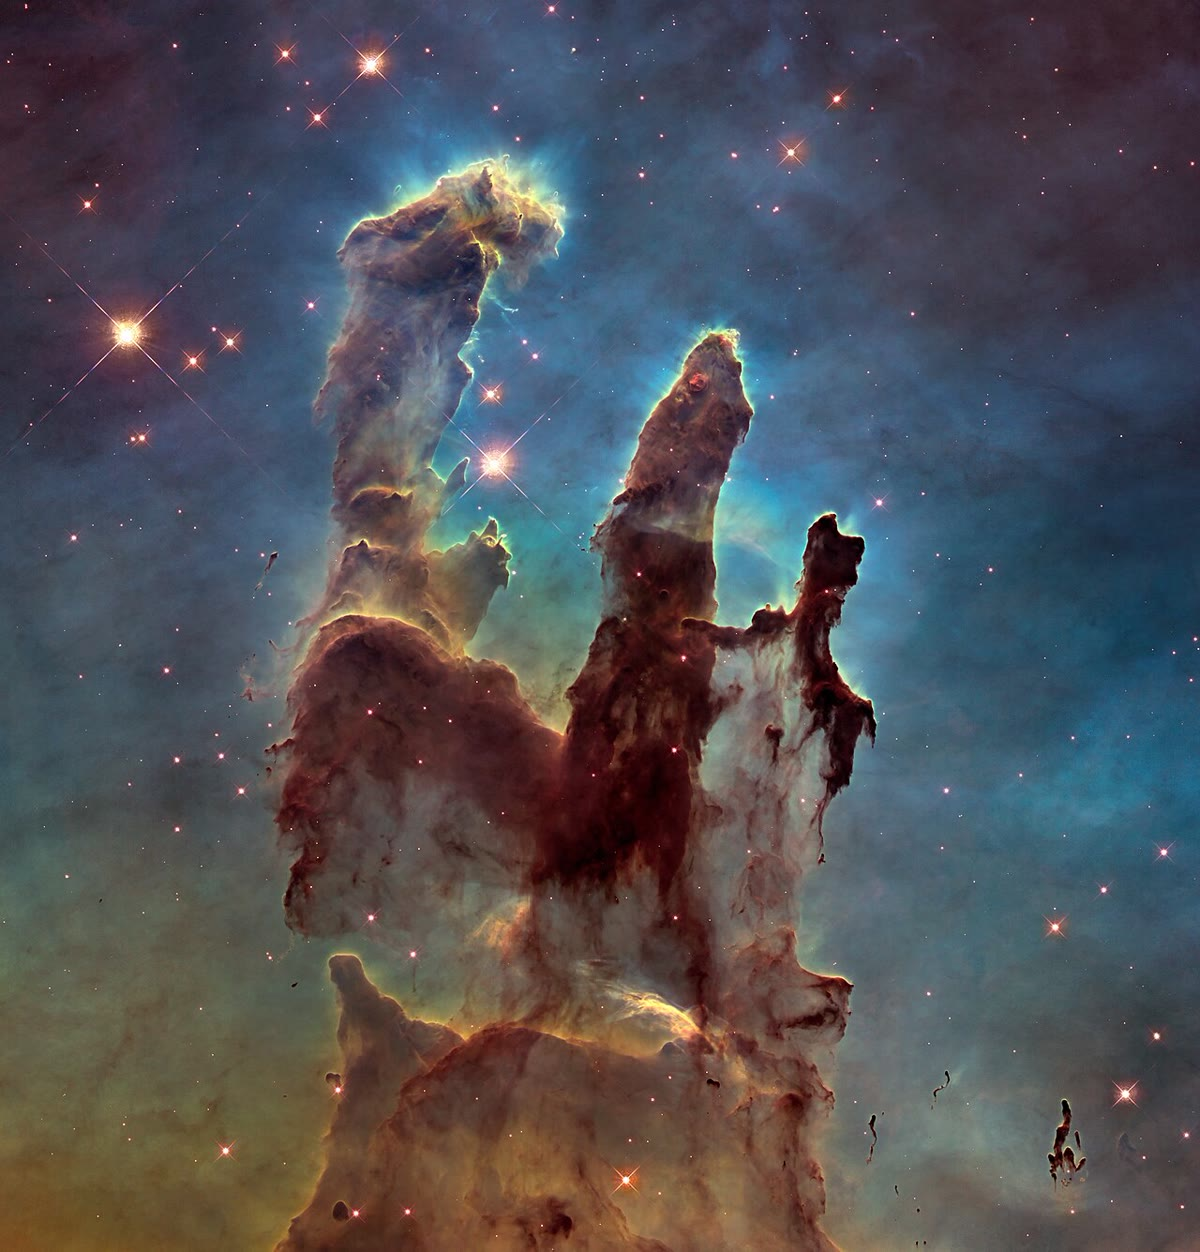
\includegraphics[width=\linewidth]{images/book4/b2-pillars-of-creation.jpg}
\end{minipage}\hfill
\begin{minipage}[c]{0.52\linewidth}
{\small ``Pilar Penciptaan'' di Nebula Elang, dicitrakan oleh Teleskop Antariksa
Hubble dalam cahaya tampak. Kolom-kolom itu adalah gas molekul dan debu yang dingin dan
padat, sepanjang beberapa tahun cahaya, yang tergerus dan disinari dari atas oleh cahaya
ultraungu bintang-bintang muda bermassa besar di luar gambar; debunya membuat kolom itu
buram. Kondensasi kecil di ujung-ujungnya sedang membentuk bintang. NASA, ESA, dan Hubble
Heritage Team (STScI/AURA), domain publik.}
\end{minipage}
\end{omfigure}

\section{Keruntuhan gravitasi}

Sebuah awan adalah keseimbangan antara dua energi: energi termal gasnya, yang mendorong
ke luar, dan energi gravitasinya, yang menarik ke dalam. Energi yang kedua tumbuh lebih
cepat terhadap massa daripada yang pertama; di atas massa tertentu, gravitasi
menang.

\begin{proposition}[Energi gravitasi bola seragam]
\label{prop:b2:ism-star-formation:grav-energy}
Sebuah bola berkerapatan seragam, bermassa $M$ dan berjari-jari $R$, memiliki
energi potensial gravitasi
\[
  U = -\frac{3}{5}\,\frac{G M^2}{R}.
\]
\end{proposition}

\begin{proof}
Bangunlah bola itu kulit demi kulit. Ketika jari-jarinya $r$, massanya
$m(r) = M r^3/R^3$; membawa sebuah kulit setebal $\mathrm dr$, bermassa
$\mathrm dm = 3M r^2\,\mathrm dr/R^3$, dari tak hingga ke permukaannya melepaskan
energi $G m(r)\,\mathrm dm/r$, karena sebuah bola menarik benda di luarnya seolah-olah
massanya terpusat di titik pusatnya (teorema kulit, fisika). Jadi
\[
  U = -\int_0^R \frac{G}{r}\,\frac{M r^3}{R^3}\,\frac{3 M r^2}{R^3}\,\mathrm dr
    = -\frac{3 G M^2}{R^6}\int_0^R r^4\,\mathrm dr = -\frac{3}{5}\,\frac{G M^2}{R}.
  \qedhere
\]
\end{proof}

Benda yang menggravitasi dirinya sendiri dan berada dalam kesetimbangan mematuhi teorema
virial: dirata-ratakan terhadap waktu, dua kali energi kinetiknya ditambah energi
gravitasinya sama dengan nol, $2K + U = 0$ (fisika, Sarjana Tahun ke-3, tempat teorema itu
diturunkan dari persamaan gerak). Untuk awan yang diam, $K$ adalah energi termal
partikel-partikelnya. Jika $2K > |U|$, gas memuai; jika $2K < |U|$, tidak ada
kesetimbangan yang dapat melawan gravitasi dan awan itu mengerut.

\begin{proposition}[Kriteria Jeans]\label{prop:b2:ism-star-formation:jeans}
Awan isotermal yang seragam, bersuhu $T$ dan berkerapatan $\rho$, yang tersusun atas
partikel bermassa rata-rata $\mu m_u$, runtuh oleh gravitasinya sendiri jika massanya
melampaui \emph{\omterm{def:b2:ism-star-formation:jeans}{massa Jeans}}
\[
  M_J = \left(\frac{5 k_{\mathrm B} T}{G\mu m_u}\right)^{3/2}
        \left(\frac{3}{4\pi\rho}\right)^{1/2},
\]
atau, secara setara, jika jari-jarinya melampaui \emph{\omterm{def:b2:ism-star-formation:jeans}{panjang Jeans}}
\[
  R_J = \left(\frac{15 k_{\mathrm B} T}{4\pi G\mu m_u\,\rho}\right)^{1/2}.
\]
Inilah \emph{kriteria Jeans}\index{kriteria Jeans}.
\end{proposition}

\begin{proof}
Awan itu berisi $N = M/(\mu m_u)$ partikel, dengan energi termal
$K = \tfrac32 N k_{\mathrm B}T = \tfrac32 M k_{\mathrm B}T/(\mu m_u)$. Menurut
\cref{prop:b2:ism-star-formation:grav-energy}, awan itu runtuh jika
$2K < \tfrac35 GM^2/R$, yaitu
\[
  \frac{3 M k_{\mathrm B} T}{\mu m_u} < \frac{3}{5}\,\frac{G M^2}{R}
  \iff M > \frac{5 k_{\mathrm B} T}{G \mu m_u}\, R .
\]
Eliminasi $R$ dengan $M = \tfrac43\pi R^3\rho$, yaitu $R = (3M/4\pi\rho)^{1/3}$:
$M^{2/3} > \frac{5 k_{\mathrm B}T}{G\mu m_u}\,(3/4\pi\rho)^{1/3}$, dan memangkatkan
kedua ruas dengan $3/2$ menghasilkan $M > M_J$. Jika yang dieliminasi adalah $M$,
$\tfrac43\pi R^3\rho > 5 k_{\mathrm B}T R/(G\mu m_u)$ menghasilkan $R^2 > 15
k_{\mathrm B}T/(4\pi G\mu m_u\rho)$, yaitu $R > R_J$.
\end{proof}

\begin{definition}[Massa Jeans, panjang Jeans]\label{def:b2:ism-star-formation:jeans}
Yang disebut \emph{massa Jeans}\index{massa Jeans} $M_J$ dan \emph{panjang
Jeans}\index{panjang Jeans} $R_J$ suatu gas dengan suhu dan kerapatan tertentu
adalah massa dan jari-jari yang di atasnya sebuah bola seragam dari gas itu
runtuh oleh gravitasinya sendiri (\cref{prop:b2:ism-star-formation:jeans}).
\end{definition}

\omterm{def:b2:ism-star-formation:jeans}{Massa Jeans} tumbuh sebanding dengan $T^{3/2}$ dan turun sebanding dengan $\rho^{-1/2}$: gas
yang dingin dan padat paling mudah runtuh. Dalam \omterm{def:b2:ism-star-formation:molecular-cloud}{awan molekul}, massa rata-rata per partikel
adalah $\mu = 2.33$ satuan massa atom, yaitu hidrogen molekul dengan satu atom helium untuk
sekitar setiap lima molekul. Pada \qty{10}{K} dan $10^4$ partikel per sentimeter
kubik, $\rho = \mu m_u n = \qty{3.87e-17}{kg.m^{-3}}$ dan
$M_J = 5.5$ massa Matahari, di dalam \omterm{def:b2:ism-star-formation:jeans}{panjang Jeans} \qty{0.13}{\parsec}:
itulah massa dan ukuran sebuah \omterm{def:b2:ism-star-formation:molecular-cloud}{inti padat}. Pada kerapatan rata-rata awan gelap,
$100$ partikel per sentimeter kubik, \omterm{def:b2:ism-star-formation:jeans}{massa Jeans} sepuluh kali lebih besar, 55
massa Matahari, dan awan bermassa \num{24000} massa Matahari seperti Taurus memuat
ratusan \omterm{def:b2:ism-star-formation:jeans}{massa Jeans} (gambar di bawah).
% ledger: kauffmann:mu, nist:u, const:kB, const:G, sun:mass, goldsmith:taurus-mass

\begin{omfigure}
\begin{tabular}{@{}c@{\hspace{3mm}}c@{}}
\begin{tikzpicture}
\begin{axis}[omrecord, width=0.455\linewidth, height=6.0cm, xmode=log, ymode=log,
  xmin=10, xmax=1e7, ymin=0.05, ymax=1e4,
  xlabel={$n$ (\unit{cm^{-3}})}, ylabel={massa Jeans (massa Matahari)},
  tick label style={font=\scriptsize}, label style={font=\small},
  legend style={font=\scriptsize, at={(0.97,0.97)}, anchor=north east, draw=none, fill=white, fill opacity=0.85}]
\fill[blue!12] (axis cs:1e4,0.5) rectangle (axis cs:1e5,5);
\node[font=\scriptsize, blue!50!black, anchor=north east] at (axis cs:1e5,0.5) {inti padat};
\addplot[very thick, blue!70!black] table[x=n, y=MJ10] {figdata/out/bachelor-2-jeans-jeans.dat};
\addlegendentry{\qty{10}{K}}
\addplot[very thick, orange!80!black] table[x=n, y=MJ20] {figdata/out/bachelor-2-jeans-jeans.dat};
\addlegendentry{\qty{20}{K}}
\addplot[very thick, red!75!black] table[x=n, y=MJ50] {figdata/out/bachelor-2-jeans-jeans.dat};
\addlegendentry{\qty{50}{K}}
\end{axis}
\end{tikzpicture}
&
\begin{tikzpicture}
\begin{axis}[omrecord, width=0.455\linewidth, height=6.0cm, xmode=log, ymode=log,
  xmin=10, xmax=1e7, ymin=0.01, ymax=20,
  xlabel={$n$ (\unit{cm^{-3}})}, ylabel={waktu jatuh bebas (Ma)},
  tick label style={font=\scriptsize}, label style={font=\small}]
\addplot[very thick, black!70] table[x=n, y=tff_Myr] {figdata/out/bachelor-2-jeans-tff.dat};
\fill[blue!12] (axis cs:1e4,0.05) rectangle (axis cs:1e5,0.5);
\addplot[very thick, black!70] table[x=n, y=tff_Myr] {figdata/out/bachelor-2-jeans-tff.dat};
\node[font=\scriptsize, blue!50!black, anchor=north] at (axis cs:3.2e4,0.05) {inti};
\end{axis}
\end{tikzpicture}
\\[2pt]
{\small (a) \omterm{def:b2:ism-star-formation:jeans}{Massa Jeans}} & {\small (b) \omterm{def:b2:ism-star-formation:free-fall}{Waktu jatuh bebas}}
\end{tabular}

\par\smallskip{\small (a) \omterm{def:b2:ism-star-formation:jeans}{Massa Jeans} terhadap kerapatan partikel untuk tiga suhu
($\mu = 2.33$). Kotak berarsir menandai massa dan kerapatan \omterm{def:b2:ism-star-formation:molecular-cloud}{inti padat} yang
teramati: pada \qty{10}{K} massanya dekat dengan \omterm{def:b2:ism-star-formation:jeans}{massa Jeans}. (b) \omterm{def:b2:ism-star-formation:free-fall}{Waktu
jatuh bebas} pada \cref{prop:b2:ism-star-formation:free-fall}: sepertiga juta
tahun pada $10^4$ partikel per sentimeter kubik, sepuluh kali lebih lama pada $10^2$.}
\end{omfigure}

Awan yang mulai runtuh menjadi makin padat, dan \omterm{def:b2:ism-star-formation:jeans}{massa Jeansnya} turun sebanding dengan
$\rho^{-1/2}$ selama awan itu tetap dingin, yang berlaku selama ia dapat memancarkan
panas kompresinya. Bagian-bagian awan kemudian menjadi tidak stabil dengan sendirinya
dan runtuh secara terpisah: awan itu \emph{terfragmentasi}. Inilah sebabnya bintang
terbentuk berkelompok dan massanya kecil dibandingkan dengan awan yang membentuknya.
Fragmentasi berhenti ketika gas menjadi terlalu padat untuk meloloskan radiasinya:
panas kompresi terperangkap, suhu naik, dan \omterm{def:b2:ism-star-formation:jeans}{massa Jeans}
berhenti turun.

Berapa lama keruntuhan berlangsung? Jika tekanan dapat diabaikan, setiap kulit awan
jatuh bebas menuju pusat.

\begin{proposition}[Waktu jatuh bebas]\label{prop:b2:ism-star-formation:free-fall}
Sebuah bola seragam berkerapatan $\rho$, mula-mula diam dan tanpa tekanan,
runtuh ke pusatnya dalam waktu
\[
  t_{\mathrm{ff}} = \left(\frac{3\pi}{32\,G\rho}\right)^{1/2},
\]
yang tidak bergantung pada jari-jarinya.
\end{proposition}

\begin{proof}
Tinjau sebuah partikel yang diam pada jarak $R$ dari pusat, di permukaan bola. Kulit-kulit
di dalamnya jatuh lebih cepat atau bersamanya, tidak pernah tertinggal, sehingga massa
$M = \tfrac43\pi R^3\rho$ yang menariknya tetap sama sepanjang jalan. Lintasannya adalah
orbit Kepler yang merosot: elips yang dipipihkan menjadi ruas garis lurus, dengan ujung
jauhnya di $R$ dan pusat tarikan di ujung lainnya, sehingga setengah sumbu panjangnya
$a = R/2$. Jatuh dari ujung jauh ke pusat memerlukan setengah periode; menurut hukum
ketiga Kepler
\[
  t_{\mathrm{ff}} = \frac12\cdot 2\pi\sqrt{\frac{(R/2)^3}{GM}}
  = \pi\sqrt{\frac{R^3}{8\,G\cdot\frac43\pi R^3\rho}}
  = \sqrt{\frac{3\pi}{32\,G\rho}} .
\]
$R$ saling meniadakan: setiap kulit bola seragam tiba di pusat pada saat yang
sama.
\end{proof}

\begin{definition}[Waktu jatuh bebas]\label{def:b2:ism-star-formation:free-fall}
Yang disebut \emph{waktu jatuh bebas}\index{waktu jatuh bebas} suatu gas berkerapatan $\rho$ adalah
$t_{\mathrm{ff}} = (3\pi/32G\rho)^{1/2}$, yaitu waktu yang diperlukan sebuah bola seragam
berkerapatan itu untuk runtuh hanya oleh gravitasinya sendiri.
\end{definition}

Untuk \omterm{def:b2:ism-star-formation:molecular-cloud}{inti padat} berkerapatan $10^4$ partikel per sentimeter kubik, \omterm{def:b2:ism-star-formation:free-fall}{waktu jatuh bebasnya}
\qty{0.34}{Ma}; untuk seluruh awan gelap berkerapatan $10^2$, \qty{3.4}{Ma}. Seandainya setiap
\omterm{def:b2:ism-star-formation:molecular-cloud}{awan molekul} di Galaksi runtuh dalam satu \omterm{def:b2:ism-star-formation:free-fall}{waktu jatuh bebas} dan berubah menjadi
bintang, Galaksi akan membentuk bintang jauh lebih cepat daripada kenyataannya: di Taurus, gas yang benar-benar berubah
menjadi bintang selama tiga juta tahun terakhir hanya sekitar satu persen awan itu.
Awan-awan itu tertahan, oleh gerak turbulen dan oleh medan magnet yang diseret oleh
bagian gas yang terionisasi, dan sebagian besar gasnya tersebar oleh
angin dan cahaya bintang-bintang masif pertama sebelum sempat runtuh: itulah sebabnya
efisiensi yang terukur di Taurus rendah.
% ledger: bt07:tff

\begin{history}[James Jeans]
James Jeans (1877--1946) pada tahun 1902 menerbitkan analisis kestabilan gas di bawah
gravitasinya sendiri yang menurunkan massa dan \omterm{def:b2:ism-star-formation:jeans}{panjang Jeans}. Ia
mempelajari pertumbuhan gelombang kerapatan kecil dalam gas seragam tak hingga dan
mendapati bahwa gelombang yang lebih panjang daripada suatu panjang kritis tidak dilawan
oleh tekanan, tetapi tumbuh: gas itu pecah menjadi kondensasi berukuran sekitar panjang
tersebut. Panjang kritisnya berbeda dari jari-jari yang diperoleh di atas hanya oleh
suatu faktor numerik; fisikanya, gravitasi melawan tekanan termal, sama saja.
\end{history}

\section{Protobintang}

Keruntuhan sebuah inti tidak seragam. Pusatnya, yang sedikit lebih padat, jatuh lebih dulu;
sebuah benda kecil, padat, dan panas terbentuk di sana dan tumbuh dengan menelan gas yang
terus menghujaninya.

\begin{definition}[Protobintang]\label{def:b2:ism-star-formation:protostar}
Yang disebut \emph{protobintang}\index{protobintang} adalah bintang yang sedang terbentuk
yang masih memperoleh sebagian besar massanya melalui akresi gas dari inti induknya;
ia bersinar oleh energi yang dilepaskan gas yang jatuh, bukan oleh fusi nuklir.
\end{definition}

Seberapa cepat sebuah \omterm{def:b2:ism-star-formation:protostar}{protobintang} tumbuh? Inti yang hampir runtuh berisi sekitar satu
\omterm{def:b2:ism-star-formation:jeans}{massa Jeans} dan jatuh dalam waktu sekitar satu \omterm{def:b2:ism-star-formation:free-fall}{waktu jatuh bebas}, sehingga massa tiba
dengan laju berorde $M_J/t_{\mathrm{ff}}$.

\begin{proposition}[Laju akresi protobintang]
\label{prop:b2:ism-star-formation:accretion}
Misalkan $c_s = (k_{\mathrm B}T/\mu m_u)^{1/2}$ adalah laju bunyi isotermal
gas sebuah inti. Perbandingan \omterm{def:b2:ism-star-formation:jeans}{massa Jeans} terhadap \omterm{def:b2:ism-star-formation:free-fall}{waktu jatuh bebas} tidak
bergantung pada kerapatan, dan
\[
  \frac{M_J}{t_{\mathrm{ff}}} \approx 10\,\frac{c_s^3}{G}:
\]
sebuah \omterm{def:b2:ism-star-formation:protostar}{protobintang} tumbuh dengan laju berorde $c_s^3/G$, yang hanya ditentukan oleh suhu
intinya.
\end{proposition}

\begin{proof}
Dengan $k_{\mathrm B}T/(\mu m_u) = c_s^2$, $M_J = 5^{3/2}\,c_s^3\,G^{-3/2}
(3/4\pi\rho)^{1/2}$ dan $t_{\mathrm{ff}} = (3\pi/32)^{1/2}(G\rho)^{-1/2}$, sehingga
\[
  \frac{M_J}{t_{\mathrm{ff}}} = 5^{3/2}\left(\frac{3}{4\pi}\right)^{1/2}
  \left(\frac{32}{3\pi}\right)^{1/2}\frac{c_s^3}{G}
  = 11.18\times0.489\times1.84\,\frac{c_s^3}{G} \approx 10\,\frac{c_s^3}{G},
\]
dan di sini $\rho$ telah saling meniadakan. Faktor itu bergantung pada bentuk inti;
model inti yang kerapatannya menurun ke arah luar, seperti yang teramati, memberikan laju
yang lebih dekat ke $c_s^3/G$ itu sendiri.
\end{proof}

Pada \qty{10}{K}, $c_s = \qty{0.19}{km.s^{-1}}$ dan $c_s^3/G$ sama dengan
\num{1.6e-6} massa Matahari per tahun: bintang seperti Matahari terhimpun dalam sekitar
\num{600000} tahun, waktu yang sebanding dengan \omterm{def:b2:ism-star-formation:free-fall}{waktu jatuh bebas} intinya.
Dalam inti yang lebih hangat, pada \qty{20}{K}, lajunya $2^{3/2} = 2.8$ kali lebih tinggi.

\begin{omfigure}
\begin{tikzpicture}[font=\scriptsize]
% panel 1: core
\begin{scope}
\shade[inner color=gray!70, outer color=gray!10] (0,0) circle (1.0);
\node[align=center] at (0,-1.45) {(1) inti padat\\$\sim\qty{0.1}{pc}$, \qty{10}{K}};
\end{scope}
% panel 2: collapse with infall arrows
\begin{scope}[xshift=3.0cm]
\shade[inner color=gray!80, outer color=gray!10] (0,0) circle (0.9);
\foreach \a in {0,45,...,315} \draw[-{Stealth[length=1.6mm]}, black!70] (\a:0.85) -- (\a:0.3);
\fill[orange!90!red] (0,0) circle (0.07);
\node[align=center] at (0,-1.45) {(2) keruntuhan\\$t_{\mathrm{ff}} \sim \qty{0.1}{Ma}$};
\end{scope}
% panel 3: protostar with disc and outflow
\begin{scope}[xshift=6.0cm]
\fill[gray!25] (0,0) ellipse (0.9 and 0.6);
\fill[brown!55] (0,0) ellipse (0.75 and 0.12);
\fill[orange!90!red] (0,0) circle (0.08);
\fill[blue!25] (0,0.1) -- (-0.22,0.95) -- (0.22,0.95) -- cycle;
\fill[blue!25] (0,-0.1) -- (-0.22,-0.95) -- (0.22,-0.95) -- cycle;
\node[align=center] at (0,-1.45) {(3) protobintang, cakram\\dan aliran keluar, $\sim\qty{0.5}{Ma}$};
\end{scope}
% panel 4: T Tauri with disc
\begin{scope}[xshift=9.0cm]
\fill[brown!55] (0,0) ellipse (0.85 and 0.1);
\fill[yellow!80!orange] (0,0) circle (0.1);
\draw[blue!40, thick] (0,0.15) -- (0,0.6); \draw[blue!40, thick] (0,-0.15) -- (0,-0.6);
\node[align=center] at (0,-1.45) {(4) bintang T Tauri\\dan cakram, 1--\qty{5}{Ma}};
\end{scope}
% panel 5: planetary system
\begin{scope}[xshift=12.0cm]
\fill[yellow!80!orange] (0,0) circle (0.12);
\foreach \r in {0.3,0.5,0.8} \draw[black!40] (0,0) ellipse ({\r} and {0.4*\r});
\fill (0.3,0) circle (0.03); \fill (-0.5,0.03) circle (0.035); \fill (0.8,0.05) circle (0.06);
\node[align=center] at (0,-1.45) {(5) bintang deret\\utama dan planet};
\end{scope}
\foreach \x in {1.4,4.4,7.4,10.4} \draw[-{Stealth}, thick, black!60] (\x,0) -- (\x+0.25,0);
\end{tikzpicture}

\par\smallskip{\small Dari \omterm{def:b2:ism-star-formation:molecular-cloud}{inti padat} ke sistem planet (skema, tidak berskala).
(1) Inti dingin di dekat \omterm{def:b2:ism-star-formation:jeans}{massa Jeans}. (2) Pusatnya runtuh lebih dulu dan sebuah \omterm{def:b2:ism-star-formation:protostar}{protobintang}
terbentuk. (3) \omterm{def:b2:ism-star-formation:protostar}{Protobintang} tumbuh melalui akresi lewat sebuah cakram, sementara \omterm{def:b2:ism-star-formation:t-tauri}{aliran keluar
bipolar} menyapu gas di sepanjang sumbu rotasi. (4) Setelah selubungnya habis, sebuah \omterm{def:b2:ism-star-formation:t-tauri}{bintang T Tauri},
yang masih mengerut, dikelilingi cakramnya. (5) Cakram telah tersebar; yang tersisa dari
zat padatnya adalah planet-planet. Waktu-waktunya berasal dari taksiran jatuh bebas dan akresi
dalam teks serta dari umur cakram pada subbab terakhir.}
\end{omfigure}

Selama berakresi, \omterm{def:b2:ism-star-formation:protostar}{protobintang} bersinar oleh energi gas yang jatuh. Begitu
selubungnya habis, ia tetap bersinar, masih tanpa fusi, dengan
mengerut.

\begin{proposition}[Pengerutan menghidupi bintang muda]
\label{prop:b2:ism-star-formation:contraction}
Bola gas yang menggravitasi dirinya sendiri, berada dalam kesetimbangan, dan mengerut
perlahan memancarkan separuh energi gravitasi yang dilepaskannya dan menyimpan separuh
lainnya sebagai panas: ia menjadi makin panas sambil kehilangan energi.
\end{proposition}

\begin{proof}
Dalam kesetimbangan, teorema virial memberikan $2K + U = 0$, sehingga energi totalnya
$E = K + U = U/2$. Jika jari-jarinya menyusut, $U$ berkurang sebesar suatu jumlah
$\Delta < 0$; maka $E$ berubah sebesar $\Delta/2$, yaitu energi yang dipancarkan
keluar, dan $K = -U/2$ berubah sebesar $-\Delta/2 > 0$: energi termal, dan karena itu
suhunya, naik sebesar separuh yang lain.
\end{proof}

\begin{definition}[Skala waktu Kelvin--Helmholtz]\label{def:b2:ism-star-formation:kh-time}
Yang disebut \emph{skala waktu Kelvin--Helmholtz}\index{skala waktu Kelvin--Helmholtz}
sebuah bintang bermassa $M$, berjari-jari $R$, dan berluminositas $L$ adalah
$t_{\mathrm{KH}} = GM^2/(RL)$, yaitu orde besar lamanya pengerutan saja dapat
memasok luminositasnya.
\end{definition}

Untuk Matahari sekarang, $t_{\mathrm{KH}} = \qty{31}{Ma}$: jauh lebih pendek daripada
umurnya, dan itulah sebabnya Matahari harus membakar hidrogen. Untuk bintang muda bermassa
satu massa Matahari, berjari-jari dua kali jari-jari Matahari, dan berluminositas dua kali
luminositasnya, nilainya \qty{8}{Ma}
(\cref{exo:b2:ism-star-formation:6}). Pengerutan berakhir ketika pusatnya cukup panas agar fusi hidrogen memasok luminositasnya: bintang itu tiba di deret utama (lihat kotak pengingat).
% ledger: sun:mass, sun:R, sun:L, const:G

\begin{definition}[Bintang T Tauri, aliran keluar bipolar]\label{def:b2:ism-star-formation:t-tauri}
Yang disebut \emph{bintang T Tauri}\index{bintang T Tauri} adalah bintang muda bermassa
kurang dari sekitar dua massa Matahari yang telah melepaskan selubungnya dan menjadi
tampak tetapi belum mencapai deret utama: ia bersinar karena pengerutan, kecerlangannya
berubah-ubah, dan biasanya dikelilingi cakram yang darinya ia masih berakresi.
Yang disebut \emph{aliran keluar bipolar}\index{aliran keluar bipolar} adalah sepasang
pancaran atau angin gas yang cepat yang dilontarkan bintang muda ke arah berlawanan di
sepanjang sumbu rotasi cakramnya.
\end{definition}

Aliran keluar membawa pergi sebagian momentum sudut gas yang diumpankan cakram ke
bintang, dan menyapu selubung di sepanjang sumbunya; bintang HL Tauri, pada akhir
tahap \omterm{def:b2:ism-star-formation:protostar}{protobintangnya}, menggerakkan aliran keluar yang sangat terkolimasi.
% ledger: alma:hltau

\section{Cakram}

Sebuah \omterm{def:b2:ism-star-formation:molecular-cloud}{inti padat} berputar, perlahan: di sepanjang inti, kecepatan gas berubah beberapa
persepuluh kilometer per sekon per parsek. Ketika inti runtuh, momentum sudutnya
kekal, dan rotasi yang lambat menjadi cepat.

\begin{proposition}[Jari-jari sentrifugal]\label{prop:b2:ism-star-formation:centrifugal}
Gas bermomentum sudut spesifik $j$ (momentum sudut per satuan massa)
yang jatuh menuju massa $M$ tidak dapat mencapai pusat: gas itu menetap pada orbit
melingkar berjari-jari
\[
  r_c = \frac{j^2}{G M}.
\]
\end{proposition}

\begin{proof}
Tanpa gesekan, momentum sudut gas yang jatuh kekal, sehingga pada
jarak $r$ laju rotasinya $v = j/r$. Gas dapat beredar pada $r$ jika
gravitasi memasok tepat percepatan sentripetalnya,
$GM/r^2 = v^2/r = j^2/r^3$, yaitu pada $r = j^2/(GM)$. Lebih ke dalam, percepatan
sentripetal yang diperlukan, $j^2/r^3$, melampaui tarikan gravitasi, dan
gas tidak dapat bergerak lebih jauh.
\end{proof}

Gas yang jatuh di sepanjang sumbu rotasi hanya memiliki sedikit momentum sudut dan langsung
menuju bintang; gas yang jatuh di bidang ekuator mempertahankan rotasinya. Gas yang jatuh
dari sisi-sisi yang berlawanan melalui lintasan yang berbeda bertumbukan di atas dan di
bawah bidang ekuator, kehilangan gerak vertikalnya, dan berkumpul menjadi cakram tipis yang
berputar dengan jari-jari sekitar $r_c$. Untuk inti berukuran
\qty{0.1}{pc} yang berputar sekali dalam sekitar dua puluh juta tahun, $r_c$ bernilai beberapa
ratus satuan astronomi (\cref{exo:b2:ism-star-formation:11}): ukuran cakram yang teramati.

\begin{definition}[Cakram protoplanet]\label{def:b2:ism-star-formation:disc}
Yang disebut \emph{cakram protoplanet}\index{cakram protoplanet} (atau
\emph{cakram protobintang}\index{cakram protobintang}) adalah cakram pipih
gas dan debu yang berotasi hampir secara Kepler di sekitar bintang muda, yang tersusun atas
materi inti induknya yang menyimpan terlalu banyak momentum sudut untuk jatuh ke
bintang; planet-planet terbentuk di dalamnya.
\end{definition}

\begin{omfigure}
\begin{minipage}[c]{0.44\linewidth}
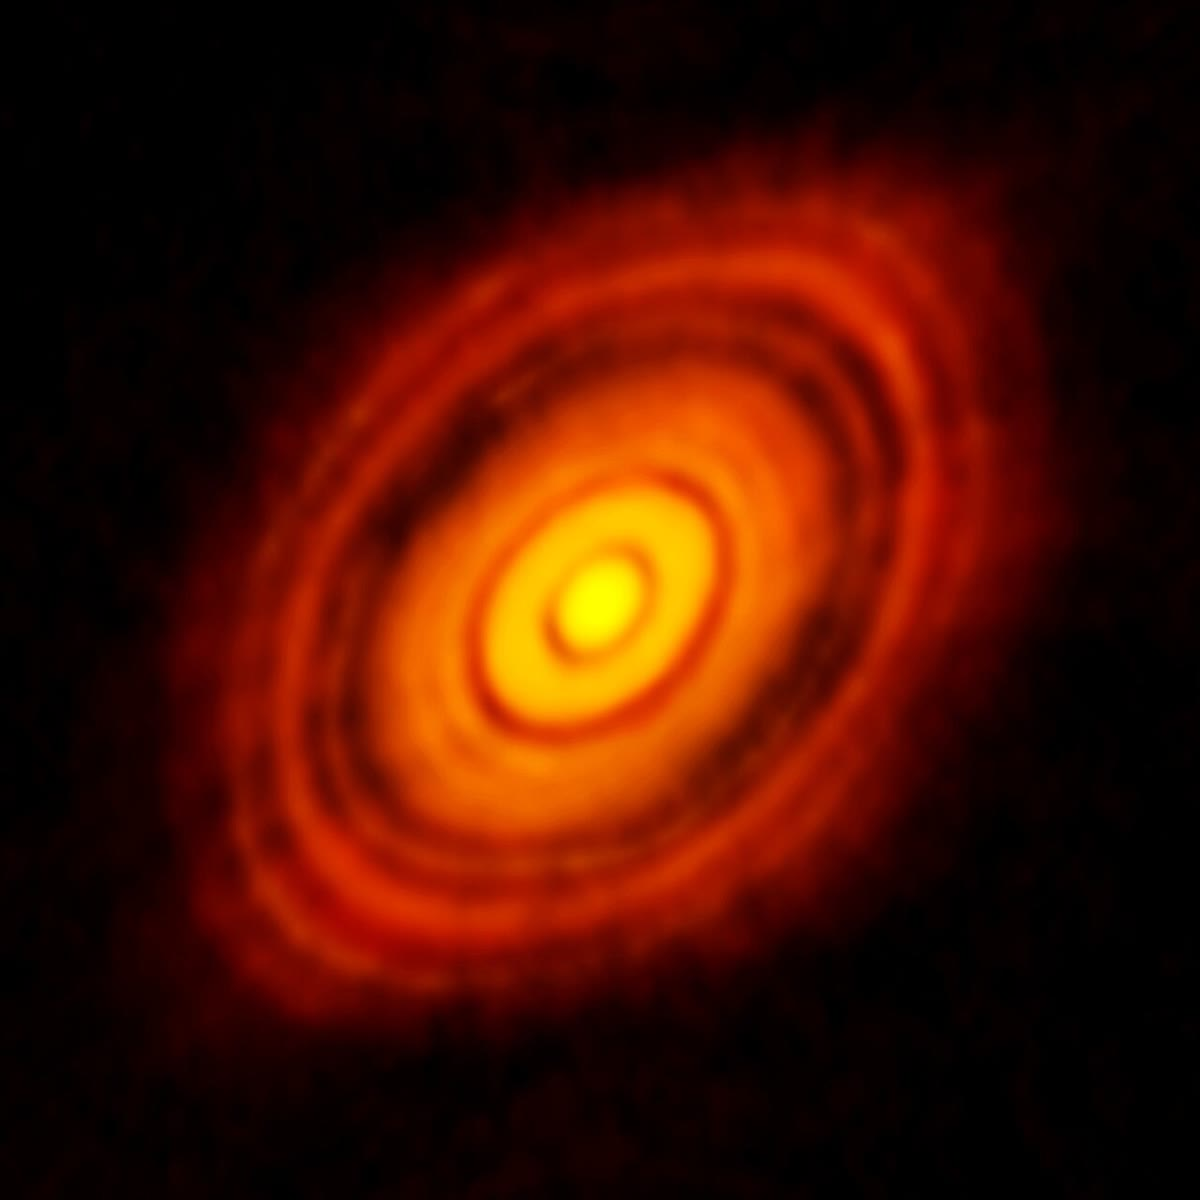
\includegraphics[width=\linewidth]{images/book4/b2-hl-tau-alma.jpg}
\end{minipage}\hfill
\begin{minipage}[c]{0.52\linewidth}
{\small Cakram bintang muda HL Tauri, \qty{140}{pc} jauhnya di Taurus, dicitrakan
oleh interferometer ALMA pada panjang gelombang sekitar satu milimeter, tempat debu dingin
bersinar. Cakram itu, berjari-jari sekitar \qty{120}{au} dan terlihat miring
\ang{47}, memperlihatkan cincin-cincin terang dan gelap selebar beberapa satuan astronomi;
sistem itu berumur paling lama satu atau dua juta tahun, dan cincin-cincinnya ditafsirkan
sebagai tanda pertama planet-planet yang menyapu lintasannya. ALMA (ESO/NAOJ/NRAO), CC BY 4.0.}
\end{minipage}
% ledger: alma:hltau
\end{omfigure}

Cakram dipanaskan oleh bintang. Sebutir debu pada jarak $r$ menyerap cahaya bintang
pada penampang lintangnya dan memancar dari seluruh permukaannya.

\begin{proposition}[Suhu butiran dalam cahaya bintang]
\label{prop:b2:ism-star-formation:grain}
Sebutir debu kecil yang berperilaku sebagai benda hitam, pada jarak $r$ dari bintang
berluminositas $L$ dan disinari hanya pada satu sisi, menetap pada suhu
\[
  T = \left(\frac{L}{16\pi\sigma r^2}\right)^{1/4},
\]
yang turun sebanding dengan $r^{-1/2}$.
\end{proposition}

\begin{proof}
Butiran bulat berjari-jari $a$ mencegat daya $\pi a^2\,L/(4\pi r^2)$
dan, pada suhu $T$, memancarkan $4\pi a^2\sigma T^4$ dari permukaannya.
Dalam kesetimbangan keduanya sama: $T^4 = L/(16\pi\sigma r^2)$; $a$ saling meniadakan.
\end{proof}

Pada jarak \qty{1}{au} dari bintang seperti Matahari, butiran itu bersuhu \qty{278}{K}; pada
\qty{5.2}{au}, tempat Jupiter mengorbit, \qty{122}{K}. Es air mengembun di tempat
butiran lebih dingin daripada sekitar \qty{180}{K} (suhu-suhu kondensasinya adalah
suhu pada \cref{ch:b2:planet-formation-meteorites}), yaitu di luar sekitar
\qty{2.4}{au}: tanda pertama dari batas, garis salju, yang memisahkan
planet berbatu dari planet es. Cakram yang sebenarnya buram, dan bidang tengahnya terlindung dari cahaya bintang langsung;
proposisi itu memberikan orde besar dan kemiringan yang benar untuk
lapisan-lapisan permukaan yang dilihat bintang.
% ledger: lodders:tc-table

Cakram tidak bertahan lama. Kelebihan inframerah, yaitu pendar debu hangat di atas apa yang
akan dipancarkan bintang itu sendiri, mengungkapkan apakah sebuah bintang masih memiliki
cakram. Menghitung bintang dengan kelebihan semacam itu di gugus-gugus berumur berbeda
memberikan fraksi bintang yang mempertahankan cakramnya sebagai fungsi waktu (gambar di
bawah): sebagian besar bintang memilikinya saat lahir, separuhnya telah kehilangannya pada
sekitar tiga juta tahun, dan hampir tidak ada yang mempertahankannya lewat dari enam juta tahun. Raksasa gas, yang harus
mengumpulkan gasnya dari cakram, harus terbentuk dalam beberapa juta tahun ini.
% ledger: haisch:disc-fractions, haisch:disc-lifetime

\begin{omfigure}
\begin{tikzpicture}
\begin{axis}[omrecord, width=0.8\linewidth, height=5.6cm, xmin=0, xmax=8.5, ymin=0, ymax=1.05,
  xlabel={umur gugus (Ma)}, ylabel={fraksi bintang bercakram},
  tick label style={font=\scriptsize}, label style={font=\small}, clip=false]
\addplot[thick, black!55, densely dashed] table[x=age, y=frac] {figdata/out/bachelor-2-jeans-discfit.dat};
\addplot[only marks, mark=*, mark size=1.8pt, blue!70!black,
  error bars/.cd, y dir=both, y explicit]
  table[x=age, y=frac, y error=err, restrict x to domain=0:10] {figdata/out/bachelor-2-jeans-discs.dat};
\node[font=\scriptsize, anchor=north west] at (axis cs:0.05,0.74) {NGC 2024};
\node[font=\scriptsize, anchor=south west] at (axis cs:1.55,0.86) {Trapesium};
\node[font=\scriptsize, anchor=south west] at (axis cs:2.35,0.71) {IC 348};
\node[font=\scriptsize, anchor=south west] at (axis cs:3.3,0.56) {NGC 2264};
\node[font=\scriptsize, anchor=south west] at (axis cs:5.1,0.15) {NGC 2362};
\node[font=\scriptsize, anchor=north east] at (axis cs:8.4,0.98) {(NGC 1960, \qty{30}{Ma}: $0.03$)};
\end{axis}
\end{tikzpicture}

\par\smallskip{\small Fraksi bintang di gugus-gugus muda yang memperlihatkan kelebihan
inframerah sebuah cakram, terhadap umur gugus (beserta galatnya), menurut Haisch, Lada
dan Lada (2001). Garis putus-putus adalah garis lurus kuadrat terkecil melalui lima
gugus termuda: garis itu mencapai $0.5$ pada \qty{3.0}{Ma} dan nol pada \qty{6.1}{Ma}
(\cref{exo:b2:ism-star-formation:12}).}
\end{omfigure}

\begin{inthelab}[Menembus debu dengan gelombang radio]
\begin{minipage}[t]{0.55\linewidth}\vspace{0pt}
Gas dan debu dingin tidak tampak oleh teleskop optik, tetapi bersinar pada panjang
gelombang milimeter, tempat atmosfer hanya transparan di atas lokasi yang tinggi dan kering.
Piringan radio sebesar rumah hanya mampu memisahkan sedikit detail pada panjang gelombang
semacam itu, sehingga para astronom menggabungkan banyak piringan: dalam sebuah interferometer,
setiap pasang antena, yang terpisah oleh suatu garis dasar, mengukur satu komponen pola
kecerahan langit, dan komputer menyusun citranya dari ratusan pasangan yang dibentuk sekitar tiga puluh antena. Resolusinya setara dengan
satu teleskop selebar garis dasar terpanjang: dengan antena yang tersebar sejauh
\qty{15}{km}, cakram HL Tauri dicitrakan dengan detail beberapa satuan astronomi pada
\qty{140}{pc}. Para operator memindahkan antena dengan kendaraan pengangkut di antara
konfigurasi-konfigurasi, dan korelator menggabungkan sinyal-sinyalnya secara waktu nyata.
\end{minipage}\hfill
\begin{minipage}[t]{0.42\linewidth}\vspace{0pt}
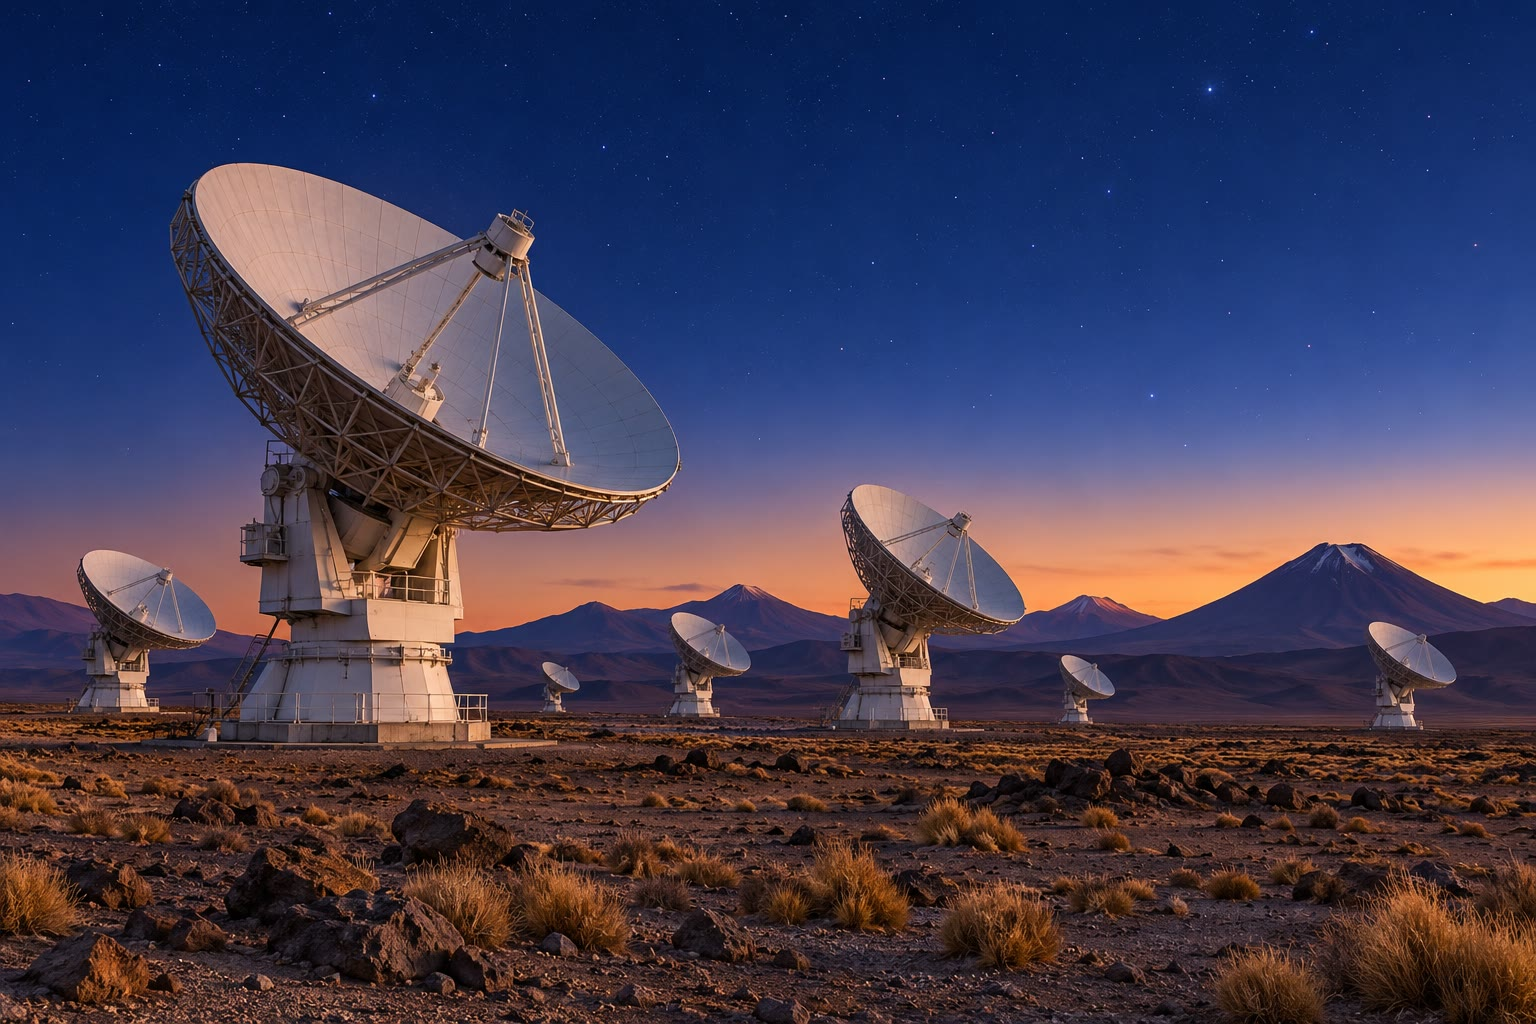
\includegraphics[width=\linewidth]{images/book4/ai/b2-radio-array.jpg}

{\scriptsize Susunan antena radio di sebuah dataran tinggi gurun saat senja
(ilustrasi buatan AI).}
\end{minipage}
% ledger: alma:hltau, alma:baselines
\end{inthelab}

\section{Latihan}

\begin{exercise}[$\star$]\label{exo:b2:ism-star-formation:1}
Kerapatan antarbintang rata-rata di dekat Matahari adalah \qty{2.7e-24}{g.cm^{-3}}. Dengan
massa atom hidrogen \qty{1.67e-24}{g}, hitunglah jumlah atom hidrogen
per sentimeter kubik. Bandingkan dengan jumlah molekul per sentimeter
kubik dalam udara pada \qty{101325}{Pa} dan \qty{288}{K} ($n = P/k_{\mathrm B}T$).
% ledger: ferriere:mean-density, const:kB
\end{exercise}

\begin{exercise}[$\star$]\label{exo:b2:ism-star-formation:2}
Dengan menggunakan nilai $M_J = 5.46$ massa Matahari pada \qty{10}{K} dan $10^4$ partikel
per sentimeter kubik, serta skala $M_J$ terhadap kerapatan, hitunglah \omterm{def:b2:ism-star-formation:jeans}{massa Jeans}
pada \qty{10}{K} dan $10^2$ partikel per sentimeter kubik. Berapa \omterm{def:b2:ism-star-formation:jeans}{massa Jeans}
yang termuat dalam awan Taurus, yang bermassa \num{24000} massa Matahari?
% ledger: goldsmith:taurus-mass
\end{exercise}

\begin{exercise}[$\star$]\label{exo:b2:ism-star-formation:3}
Hitunglah laju bunyi isotermal $c_s = (k_{\mathrm B}T/\mu m_u)^{1/2}$ gas
molekul ($\mu = 2.33$, $m_u = \qty{1.661e-27}{kg}$) pada \qty{10}{K} dan pada
\qty{100}{K}. Berapa lama gelombang bunyi menyeberangi inti berjari-jari
\qty{0.1}{pc} pada \qty{10}{K}, dalam juta tahun?
% ledger: kauffmann:mu, nist:u, iau:parsec
\end{exercise}

\begin{exercise}[$\star$]\label{exo:b2:ism-star-formation:4}
Hitunglah \omterm{def:b2:ism-star-formation:free-fall}{waktu jatuh bebas} \omterm{def:b2:ism-star-formation:molecular-cloud}{inti padat} berkerapatan $10^5$ partikel per sentimeter
kubik dan awan gelap berkerapatan $10^2$ ($\mu = 2.33$). Mana yang runtuh
lebih cepat, dan dengan faktor berapa?
\end{exercise}

\begin{exercise}[$\star\star$]\label{exo:b2:ism-star-formation:5}
Tunjukkan bahwa $M_J$ dapat ditulis $M_J = 5^{3/2}\,(3/4\pi)^{1/2}\,c_s^3\,G^{-3/2}\rho^{-1/2}$.
Pada suhu tetap, dengan faktor berapa kerapatan sebuah inti harus naik agar \omterm{def:b2:ism-star-formation:jeans}{massa Jeansnya}
menjadi separuh? Pada kerapatan tetap, dengan faktor berapa \omterm{def:b2:ism-star-formation:jeans}{massa Jeans} berubah jika
inti itu menghangat dari \qty{10}{K} menjadi \qty{20}{K}?
\end{exercise}

\begin{exercise}[$\star\star$]\label{exo:b2:ism-star-formation:6}
Sebuah bintang muda memiliki massa Matahari, dua kali jari-jarinya, dan dua kali luminositasnya
($M_\odot = \qty{1.989e30}{kg}$, $R_\odot = \qty{6.96e8}{m}$,
$L_\odot = \qty{3.83e26}{W}$). Hitunglah waktu Kelvin--Helmholtz-nya dalam juta
tahun, dan bandingkan dengan umur cakram.
% ledger: sun:mass, sun:R, sun:L
\end{exercise}

\begin{exercise}[$\star\star$]\label{exo:b2:ism-star-formation:7}
Hitunglah laju akresi $c_s^3/G$ sebuah \omterm{def:b2:ism-star-formation:protostar}{protobintang} dalam inti bersuhu \qty{10}{K}, dalam
massa Matahari per tahun, dan waktu yang diperlukannya untuk menghimpun satu massa Matahari.
Jawablah pertanyaan yang sama untuk inti bersuhu \qty{20}{K}.
\end{exercise}

\begin{exercise}[$\star\star$]\label{exo:b2:ism-star-formation:8}
Dengan \cref{prop:b2:ism-star-formation:grain} dan $L_\odot = \qty{3.83e26}{W}$,
hitunglah jarak dari Matahari, dalam satuan astronomi, tempat sebutir debu
mencapai \qty{1300}{K}, mendekati suhu mengembunnya silikat-silikat yang umum
(\cref{ch:b2:planet-formation-meteorites}), serta
suhu butiran pada jarak Jupiter, \qty{5.2}{au}.
% ledger: sun:L, const:sigma, const:au
\end{exercise}

\begin{exercise}[$\star\star$]\label{exo:b2:ism-star-formation:9}
Gas cakram HL Tauri berotasi mengelilingi bintang bermassa sekitar \num{1.3} massa
Matahari. Hitunglah laju Kepler dan periode orbitnya pada \qty{100}{au}.
Jika sistem itu berumur satu juta tahun, berapa kali gas pada
\qty{100}{au} telah berputar sejak bintang itu terbentuk?
% ledger: alma:hltau
\end{exercise}

\begin{exercise}[$\star\star\star$]\label{exo:b2:ism-star-formation:10}
Tentukan energi gravitasi sebuah bola berjari-jari $R$ yang kerapatannya
turun sebagai $\rho(r) = \rho_0 R/r$, dan bandingkan dengan energi gravitasi bola seragam
bermassa dan berjari-jari sama. Apakah pemusatan massa ke arah pusat membuat
awan itu lebih mudah atau lebih sulit ditopang oleh energi termalnya?
\end{exercise}

\begin{exercise}[$\star\star\star$]\label{exo:b2:ism-star-formation:11}
Sebuah inti berjari-jari \qty{0.1}{pc} berotasi sebagai benda tegar dengan laju sudut
$\Omega = \qty{1e-14}{rad.s^{-1}}$. Hitunglah periode rotasinya, momentum sudut
spesifik $j = \Omega R^2$ gas di ekuatornya, dan jari-jari sentrifugal
gas itu di sekitar bintang bermassa satu massa Matahari, dalam satuan astronomi.
Mengapa gas dari bagian dalam inti mendarat lebih dekat ke bintang?
\end{exercise}

\begin{exercise}[$\star\star\star$]\label{exo:b2:ism-star-formation:12}
Fraksi cakram lima gugus termuda pada gambar di subbab terakhir
adalah $0.85$, $0.80$, $0.65$, $0.52$, dan $0.12$ pada 0.3, 1.5, 2.3, 3.2, dan
\qty{5.0}{Ma}. Cocokkan garis lurus kuadrat terkecil $f = a - bt$ secara manual
(hitung rata-ratanya, lalu $\sum(t - \bar t)(f - \bar f)$ dan
$\sum(t - \bar t)^2$). Pada umur berapa garis itu mencapai setengah, dan nol? Mengapa
garis lurus merupakan model yang buruk lewat dari umur itu?
% ledger: haisch:disc-fractions
\end{exercise}

\section{Soal: Sebuah inti di awan Aldra}

\begin{problem}[{Soal akhir pekan --- massa dan kestabilan sebuah inti padat yang dibaca dari
peta debu, kelahiran protobintangnya, dan ukuran cakramnya}]
\label{pb:b2:ism-star-formation:1}
% values: calc/ch01.py
% ledger: kauffmann:mu, nist:u, iau:parsec, const:G, const:kB, sun:mass, sun:R, sun:L, const:au, const:sigma, bt07:cores, alma:hltau
Awan Aldra adalah awan gelap rekaan. Peta milimeter debunya
memperlihatkan inti bundar berjari-jari \qty{0.08}{pc}, dengan kerapatan kolom rata-rata
$N(\ce{H2}) = \num{1.5e22}$ molekul hidrogen per sentimeter persegi. Sebuah
garis amonia memberikan suhu gas, \qty{10}{K}, dan gradien kecepatan
\qty{0.4}{km.s^{-1}} per parsek di sepanjang inti, yang ditafsirkan sebagai rotasi
benda tegar. Gunakan $G = \qty{6.674e-11}{m^3.kg^{-1}.s^{-2}}$,
$k_{\mathrm B} = \qty{1.381e-23}{J.K^{-1}}$, $m_u = \qty{1.661e-27}{kg}$,
\qty{1}{pc} $= \qty{3.086e16}{m}$, \qty{1}{au} $= \qty{1.496e11}{m}$, satu tahun
\qty{3.156e7}{s}, $M_\odot = \qty{1.989e30}{kg}$, $R_\odot = \qty{6.96e8}{m}$,
$L_\odot = \qty{3.83e26}{W}$, $\sigma = \qty{5.67e-8}{W.m^{-2}.K^{-4}}$; massa per
molekul hidrogen, termasuk helium, adalah $2.8\,m_u$, dan massa rata-rata
per partikel $2.33\,m_u$.

\medskip
\noindent\textbf{Bagian I --- Massa dan kerapatan.}
\begin{enumerate}
  \item Ubahlah jari-jari inti ke dalam meter.
  \item Hitunglah massa per meter persegi kolom itu, $2.8\,m_u N$.
  \item Simpulkan massa inti, dalam kilogram dan dalam massa Matahari.
  \item Hitunglah volume dan kerapatan rata-ratanya.
  \item Hitunglah jumlah partikel per sentimeter kubik.
  \item Apakah ini \omterm{def:b2:ism-star-formation:molecular-cloud}{inti padat} dalam arti tabel di subbab kedua?
\end{enumerate}

\noindent\textbf{Bagian II --- Kestabilan.}
\begin{enumerate}[resume]
  \item Hitunglah \omterm{def:b2:ism-star-formation:jeans}{massa Jeans} gas inti itu, dalam massa Matahari.
  \item Berapa \omterm{def:b2:ism-star-formation:jeans}{massa Jeans} yang dimuat inti itu? Apakah inti itu stabil?
  \item Hitunglah \omterm{def:b2:ism-star-formation:jeans}{panjang Jeans} dan bandingkan dengan jari-jari inti.
  \item Berapa \omterm{def:b2:ism-star-formation:jeans}{massa Jeans} seandainya gas itu bersuhu \qty{20}{K}? Apakah
        inti itu masih akan runtuh?
  \item Hitunglah \omterm{def:b2:ism-star-formation:free-fall}{waktu jatuh bebas} inti itu, dalam ribuan tahun.
  \item Bandingkan dengan waktu yang diperlukan gelombang bunyi untuk menyeberangi inti. Proses
        mana yang lebih cepat, dan apa artinya?
\end{enumerate}

\noindent\textbf{Bagian III --- Protobintang.}
\begin{enumerate}[resume]
  \item Hitunglah laju bunyi di dalam inti.
  \item Hitunglah laju akresi $c_s^3/G$, dalam massa Matahari per tahun.
  \item Hitunglah waktu yang diperlukan untuk menghimpun satu massa Matahari dengan laju ini.
  \item Jika sepertiga inti berakhir sebagai bintang, berapa bintang bermassa satu massa
        Matahari yang dapat dibentuknya?
  \item Setelah selubungnya habis, bintang itu bermassa satu massa Matahari, berjari-jari tiga
        jari-jari Matahari, dan berluminositas empat luminositas Matahari. Hitunglah waktu Kelvin--Helmholtz-nya.
  \item Apakah waktu itu lebih panjang atau lebih pendek daripada waktu akresi? Bintang jenis apakah
        ia saat itu?
\end{enumerate}

\noindent\textbf{Bagian IV --- Cakram.}
\begin{enumerate}[resume]
  \item Ubahlah gradien kecepatan menjadi laju sudut $\Omega$, dalam
        \unit{rad.s^{-1}}.
  \item Hitunglah momentum sudut spesifik $j = \Omega R^2$ gas di
        ekuator inti.
  \item Hitunglah jari-jari sentrifugalnya di sekitar bintang bermassa satu massa Matahari, dalam
        satuan astronomi.
  \item Hitunglah suhu sebutir debu pada jarak \qty{1}{au} dan \qty{30}{au}
        dari bintang berluminositas satu luminositas Matahari.
  \item Di manakah garis salju cakram ini, jika es air bertahan di bawah
        \qty{180}{K}?
  \item Nyatakan waktu yang diperlukan untuk menghimpun bintang pada pertanyaan 15, angka
        kunci soal ini, dalam ribuan tahun, dan bandingkan dengan
        \omterm{def:b2:ism-star-formation:free-fall}{waktu jatuh bebas} pada pertanyaan 11.
\end{enumerate}
\end{problem}
